This section concerns the estimator used for estimation of the consumer demand flows.

\subsection{Estimator Objective}
The LQR controller relies on knowledge of the current  consumer demand flows. The consumption flow is not measured directly but can be calculated from the combined measurements of tank flow $d_\tau$ and pump flows $d_p$. If no leakage is present, all nodal demands sum to zero (mass conservation) and thus $d_c = d_p + d_\tau$. Noise will be present on all flow sensor measurements which will affect LQR controller performance. Thus it is favourable to estimate the actual underlying consumer flow, attenuating measurement noise.

\subsection{Estimator Model}
An initial solution for estimating the consumer flow is to utilise the full fast dynamic system matrix. This requires the ability to accurately model the full system, which has been done in this case, but is not feasible for real, large WDNs. Therefore another solution is explored.

If prior knowledge of the behaviour of the process is available, this can be taken advantage of. A new state space model describing the behaviour of the process can be made. The consumption can be approximated by a truncated Fourier series. From the consumption pattern data reviewed in \cref{sec:kalman_imp} it becomes apparent that a fourth-order approximation is appropriate. This approximation is seen in \cref{eq:consump_pattern_actual}.

\begin{equation} \label{eq:consump_pattern_actual}
	d_{c_{approx}}(t) = k_0 + k_1 cos(\omega t + \phi_1) + k_2 cos(2\omega t \phi_2) + k_3 cos(3\omega t + \phi_3) + k_4 cos(4\omega t + \phi_4)
\end{equation}

The principles behind development and utilisation of a such Fourier-series model are adequately understood from a second-order example. Thus only a model of this order is further examined here. Such a model can be seen in \cref{eq:consump_pattern}. 

\begin{equation} \label{eq:consump_pattern}
	d_{c_estimate} = K + k_1 cos(\omega t) + k_2 cos(2\omega t)
\end{equation}



This process model output should be achievable as a combination of states. As such the following states are chosen:

\begin{equation} \label{eq:consump_x}
	x_{desired} =  \begin{bmatrix}
		x_1 \\
		x_2 \\
		x_3
	\end{bmatrix}
	=
	\begin{bmatrix}
		K \\
		k_1 cos(\omega t) \\
		k_2 cos(2\omega t)
	\end{bmatrix}
\end{equation}

As with any state-space system these states need to be expressed in terms of their derivatives ($\dot x = Ax$) which are:

\begin{equation} \label{eq:consump_x_deriv_s}
	\dot x_{desired}  = \begin{bmatrix}
		\dot x_1 \\
		\dot x_2 \\
		\dot x_3
	\end{bmatrix}
	=
	\begin{bmatrix}
		0 \\
		- \omega k_1 sin(\omega t) \\
		- 2\omega k_2 sin(2\omega t)
	\end{bmatrix}
\end{equation}

No linear combination of our current states can yield this derivative. Thus we need to expand our states such that this can be achieved. Our state vector expands to:

\begin{equation} \label{eq:consump_x_l}
		x =  \begin{bmatrix}
			x_1 \\
			x_2 \\
			x_3 \\
			x_4 \\
			x_5
		\end{bmatrix}
		=
		 \begin{bmatrix}
		K \\
		k_1 cos(\omega t) \\
		k_1 sin(\omega t) \\
		k_2 cos(2 \omega t) \\
		k_2 sin(2 \omega t) 
	\end{bmatrix}
\end{equation}

Which has the state derivative:

\begin{equation} \label{eq:consump_x_deriv_l}
	\dot x =  \begin{bmatrix}
		\dot x_1 \\
		\dot x_2 \\
		\dot x_3 \\
		\dot x_4 \\
		\dot x_5
	\end{bmatrix}
	=
	\begin{bmatrix}
		0 \\
		- \omega k_1 sin(\omega t) \\
		\omega k_1 cos(\omega t) \\
		- 2\omega k_2 sin (2 \omega t) \\
		2 \omega k_1 cos(2 \omega t)
	\end{bmatrix}
\end{equation}


The system matrix then needs to be:

\begin{equation} \label{eq:consump_A}
A = 
\begin{bmatrix}
	0 & 0 & 0 & 0 & 0 \\
	0 & 0 & -\omega & 0 & 0 \\
	0 & \omega & 0 & 0 & 0 \\
	0 & 0 & 0 & 0 & -2\omega \\
	0 & 0 & 0 & 2\omega & 0 
\end{bmatrix}
\end{equation}

For $y = Cx$ to be equal to \cref{eq:consump_pattern} the C-matrix becomes: 

\begin{equation}
	C = \begin{bmatrix} 1 & 1 & 0 & 1 & 0 \end{bmatrix}
\end{equation}

If one wishes have a signal model of greater harmonic orders, a concatenation of e.g. the first order harmonic signal model, like seen in \cref{eq:first_order_signal_model}, can be performed for an arbitrary amount of harmonics. 

\begin{equation}\label{eq:first_order_signal_model}
	\begin{gathered}
		\dot{x} = A_\delta x =  \begin{bmatrix}0 & 0 & 0 \\ 0 & 0 & -\omega \\ 0 & \omega & 0	\end{bmatrix}x \\
		y = C_\delta x = \begin{bmatrix} 1 & 1 & 0 \end{bmatrix} x
	\end{gathered}
\end{equation}

Such a concatenation would, for a second-order approximation, look like so:

\begin{equation}\label{eq:DisturbanceVectorCase}
	\begin{gathered}
		\begin{bmatrix} K \\ \dot{x}_1 \\ \dot{x}_2 \end{bmatrix} = \begin{bmatrix} 
			0 & 0 & 0 \\
			0 & A_{\delta_1} & 0 \\ 
			0 & 0 & A_{\delta_2}
		\end{bmatrix} \begin{bmatrix} K \\ x_1 \\ x_2 \end{bmatrix},
		\quad y = C_\delta \begin{bmatrix} K \\ x_1 \\ x_2 \end{bmatrix} \\
		x_1, x_2 \in \mathbb{R}^{2\times1} \\
		\forall i: \ A_{\delta_i} \in \mathbb{R}^{2\times2} \\
		C_\delta \in \mathbb{R}^{1\times2n+1}
	\end{gathered}
\end{equation}

\subsection{Estimator Type}
Since the disturbance can be described as a linear system, we need a linear estimator. The optimal affine (and hence also linear) estimator is the Kalman filter, if the following conditions are fulfilled

\begin{enumerate}
	\item The consumer flow disturbance can be modelled as a dynamic system excited by white zero-mean Gaussian noise
	\item The flow measurement noise can be considered white zero-mean Gaussian noise
	\item The model uncertainty can be modelled as zero-mean white Gaussian noise
	\item The measurement noise and model uncertainty are uncorrelated
\end{enumerate}

It is the optimal affine estimator given some assumptions about the precision of the model of the process and the knowledge of the process and measurement noise, which is further described in \cref{sec:the_kalman_filter}.





\subsection{The Kalman Filter} \label{sec:the_kalman_filter}
The Kalman filter is an optimal estimator, where the optimality criterion with respect to the Mean Squared Error (MSE) of the residual $x-\hat{x}$.
It estimates an unknown process by a combination of a system model and a measurement that is related to the unknown processes. 

The Kalman filter recursively finds the optimal \textit{Kalman gain} for the given system to minimize the residual MSE. Finding the optimal gain relies on assuming that the model and measurement noise are uncorrelated white noise processes with known covariances. 

The performance of the Kalman filter relies heavily on the guess of the covariance of measurement and model noise. This means in practice that an online tuning of covariances is desirable to avoid bad guesses of the covariances \cite[p. 232]{Doraiswami2014}.

\subsubsection{Mathematical Formulation of the Kalman Filter in State Space}
The Kalman Filter described in this report will based on a discrete time state space representation: 

\begin{align}
	&{x}(k+1) = {A}{x}(k) + {B}{u}(k) + {w}(k)  \label{eq:KalmanSystemEquations} \\
	&{y}(k) = {C}{x}(k)+{v}(k) 
\end{align}
where 
\begin{align*}
	&\text{${x}(k)$ is the state vector at time index k,					}	\\[-1em]
	&\text{${u}(k)$ is the input at time index k, 						}	\\[-1em]
	&\text{${w}(k) \sim \mathcal{N}(0, Q)$ is the model noiseat time index k,			}	\\[-1em]
	&\text{${v}(k) \sim \mathcal{N}(0, R)$ is the measurement noise at time index k,		}	\\[-1em]
	&\text{${y}(k)$ is the observable output, 							}	\\[-1em]
	&\text{{A} is the state transition matrix,							}	\\[-1em]
	&\text{{B} is the control-input matrix,								}	\\[-1em]
	&\text{{C} is the observation matrix. 								}	\\[-1em]
\end{align*}

To simplify the presentation for the readers of this report the Kalman equations will be presented in the form of 8 equations, after which they can be combined to yield the traditional and more dense form of 5 equations.
The Kalman equations will further be divided into two phases: the prediction stage and the update stage. 

{Prediction stage}
\begin{align}
	&\hat{{x}}	(k|k-1) = {A} 	\hat{{x}}(k-1|k-1) + {B}{u}(k-1)  				\label{eq:Kalman_pred_state} 	\\
	&\hat{{y}}	(k|k-1) = {C}	\hat{{x}}(k|k-1)										\label{eq:Kalman_pred_output} 	\\
	&{P}			(k|k-1) = {A}	{P}(k-1|k-1){A}^T+{Q} 								\label{eq:Kalman_pred_cov} 		
\end{align}
where 
\begin{align*}
	&\text{$\hat{{x}}	(k|k-1)$ 	is the state prediction 			estimate at time index $k$ 		given all $ k-1 $ samples		}	\\[-1em]
	&\text{$\hat{{x}}	(k-1|k-1)$ 	is the state 						estimate at time index $k-1$ 	given all $ k-1 $ samples		}	\\[-1em]
	&\text{$\hat{{y}}	(k|k-1)$ 	is the output prediction 			estimate at time index $k$ 		given all $ k-1 $ samples		}	\\[-1em]
	&\text{${P}			(k|k-1)$ 	is the predicted estimate  covariance matrix at time index $k$ 		given all $ k-1 $ samples		}	\\[-1em]
	&\text{${P}			(k-1|k-1)$ 	is the updated estimate    covariance matrix at time index $k-1$ 	given all $ k-1 $ samples		}	\\[-1em]
	&\text{${Q}$						is the model/process noise covariance matrix														}	\\[-1em]
\end{align*}

All three prediction equations predicts the a priori $k$th (next) estimate based on the $k-1$ previous samples and the model knowledge.\\

\textbf{Update Stage}

\begin{align}
	&{e}			(k) 		= {y}(k) - \hat{{y}}(k|k-1)							\label{eq:Kalman_upd_inno}			\\
	&{S}			(k) 		= {C}{P}(k|k-1){C}^T + {R}				\label{eq:Kalman_upd_inno_cov}		\\
	&{K}			(k) 		= {P}(k|k-1){C}^T{S}^{-1}(k)					\label{eq:Kalman_upd_kalman_gain}	\\
	&\hat{{x}}	(k|k) 		= \hat{{x}}(k|k-1) + {K}(k){e}(k) 				\label{eq:Kalman_upd_est_state}		\\
	&{P}			(k|k) 		= ({I} - {K}(k){C}){P}(k|k-1)			\label{eq:Kalman_upd_est_cov}
\end{align}
where 
\begin{align*}
	&\text{${e}		(k)$ 		is the innovation term for time index 					$ k $													}	\\[-1em]
	&\text{${y}		(k)$ 		is the observed output at time index 					$ k $													}	\\[-1em]
	&\text{${S}		(k)$ 		is the innovation covariance for time index 			$ k $											}	\\[-1em]
	&\text{${R}$ 				is the observation noise covariance																}	\\[-1em]
	&\text{${K}		(k)$ 		is the Kalman gain for time index 						$ k $													}	\\[-1em]
	&\text{$\hat{{x}}(k|k)$ 	is the estimate of the state vector at time index 			$ k $ given all 	$ k$ samples	}	\\[-1em]
	&\text{${P}		(k|k)$ 	is the updated estimate covariance matrix at time index 	$ k $ given all 	$ k$ samples		}	\\[-1em]
	&\text{${I}$ 				is the identity matrix																				}	\\[-1em]			
\end{align*}

All the equations in the update stage estimates the posteriori estimate of the $ k $ sample based on all $ k^{th} $ samples and the model knowledge. A few expressions to give some intuitions to what the equations actually represent. The estimate covariance, the prediction covariance and innovation covariance can respectively be represented as 

\begin{align}
	&{P}(k|k) 	= \text{cov}({x}(k)-	\hat{{x}}(k|k))	\\
	&{P}(k|k-1) 	= \text{cov}({x}(k)-	\hat{{x}}(k|k-1)) 		\\
	&{S}(k) 		= \text{cov}({e}(k)) 
\end{align}

\textbf{Compact Form}\\
Now collecting some of the above equations gives the more compact form of the Kalman equations.
\Cref{eq:Kalman_pred_state,eq:Kalman_pred_cov} remain in the same form, but omitting $ {Bu}(k-1) $ yields \cref{eq:Kalman_pred_state_compact} and \cref{eq:Kalman_pred_cov_compact}. $ {Bu}(k-1) $ can be omitted as it is not part of the system model in \cref{eq:first_order_signal_model}.\\
\Cref{eq:Kalman_upd_inno_cov,eq:Kalman_upd_kalman_gain} are combined yielding \cref{eq:Kalman_upd_kalman_gain_compact}. \Cref{eq:Kalman_pred_output} is combined with \cref{eq:Kalman_upd_inno} and \cref{eq:Kalman_upd_est_state} yielding \cref{eq:Kalman_upd_est_state_compact}, while \cref{eq:Kalman_upd_est_cov} remains the same. All these combined presents the Kalman equations as in \cite{Bozic1994}\\

\textbf{Prediction}
\begin{align}
	&\hat{{x}}	(k|k-1) = {A} \hat{{x}}	(k-1|k-1) 		\label{eq:Kalman_pred_state_compact} 	\\
	&{P}			(k|k-1) = {A}{P}			(k-1|k-1){A}^T+{Q} 				\label{eq:Kalman_pred_cov_compact} 		
\end{align}
\textbf{Update}
\begin{align}
	&{K}			(k) 		= {P}				(k|k-1){C}^T({C}{P}	(k|k-1)	{C}^T + {R})^{-1}										\label{eq:Kalman_upd_kalman_gain_compact} \\
	&\hat{{x}}	(k|k) 	= \hat{{x}}			(k|k-1) + {K}						(k)	({y}		(k) - {C}\hat{{x}}		(k|k-1)) 	\label{eq:Kalman_upd_est_state_compact} \\
	&{P}			(k|k) 	= ({I} - {K}	(k){C}){P}					(k|k-1)																		\label{eq:Kalman_upd_est_cov_compact}
\end{align}


\subsubsection{LTI Kalman Filter}
If we assume that the covariances and system are time invariant, i.e. $\forall k: \ \{A(k),B(k),Q(k),R(k)\} = \{A,B,Q,R\} $, the estimate covariance and Kalman gain can be calculated offline as they don't depend on measurements, only on $ {A}, {C}, {Q}, {R} $. As such, the Kalman filter itself becomes an LTI filter. The steady state prediction covariance can be found by solving its Algebraic Riccati equation (ARE) - it will now be derived in the discrete form.\\


In steady-state where $k \rightarrow \infty$ we can assume that ${P}(k|k) = {P}(k-1|k-1) $. Furthermore the prediction covariance, the estimation covariance, and the Kalman gain converge to a constant value:
\begin{equation}
	\begin{gathered}
		\lim_{k \to \infty}	{P}(k|k-1) =  \Pi \\
		\lim_{k \to \infty} {P}(k|k) = P \\
		\lim_{k \to \infty} {K}(k) = K
	\end{gathered}
\end{equation}
Equations \cref{eq:Kalman_upd_kalman_gain_compact}, \cref{eq:Kalman_upd_est_state_compact} and \cref{eq:Kalman_upd_est_cov_compact} are rewritten with their steady state counterparts:
\begin{align}
	& K = \Pi {C}^T ({C} \Pi {C}^T + {R})^{-1} \label{eq:ss_kalman_kalman_gain} \\
	& P = ({I} - K {C}) \Pi \label{eq:ss_kalman_mse} \\
	& \Pi = {A}P{A}^T + {Q} \label{eq:ss_kalman_mse_pred}
\end{align}
We go on the hunt for the damened Riccati equation of $\Pi$. We substitute RHS of \cref{eq:ss_kalman_mse} into \cref{eq:ss_kalman_mse_pred}.
\begin{equation}
	\begin{split}\label{eq:ss_kalman_udledning1}
		\Pi 	& = {A}P A^T + Q \\
		& = {A} ({I}-K{C}) \Pi {A}^T + {Q}\\
		& = {A} \Pi {A}^T - {A} K {C} \Pi  {A}^T + {Q}\\
		\end{split}
\end{equation}
We now substitute RHS of \cref{eq:ss_kalman_kalman_gain} in for $K$ in \cref{eq:ss_kalman_udledning1} and factorize respectively ${A}$ and $ {A}^T $.
\begin{equation}
	\begin{split}\label{eq:ss_kalman_udledning2}
		\Pi & = {A} \Pi {A}^T - {A} \Pi {C}^T ({C} \Pi {C}^T + {R})^{-1} {C} \Pi {A}^T + {Q}\\
		& = {A} (\Pi - \Pi {C}^T ({C} \Pi {C}^T + {R})^{-1} {C} \Pi) {A}^T + {Q}\\
	\end{split}
\end{equation}
And let The Matrix Inversion lemma \cref{eq:ss_kalman_MatrixInversionLemma} be used to further simplify whats left in the parenthesis of RHS of \cref{eq:ss_kalman_udledning2} by letting
\begin{equation}
		{A}^{-1} = \Pi, {B} = {C}^T, {C}^{-1} = {R}, {D} = {C} \label{eq:ss_kalman_udledning3}
\end{equation}
enables 
\begin{align}
		({A}+{BCD})^{-1} &= {A}^{-1} - {A}^{-1}{B} ({D}{A}^{-1}{B}+{C}^{-1})^{-1}{D}{A}^{-1} \\ \label{eq:ss_kalman_MatrixInversionLemma}
		(\Pi^{-1} + {C}^T {R}^{-1} {C})^{-1} &= (\Pi - \Pi {C}^T ({C} \Pi {C}^T + {R})^{-1} {C} \Pi)
\end{align}
yielding the desired result: The Algebraic Riccati equation in a compact form, \cref{eq:ss_kalman_udledning4}.
\begin{equation}
	\begin{split}\label{eq:ss_kalman_udledning4}
		&\Pi = {A} (\Pi^{-1} + {C}^T {R}^{-1} {C})^{-1} {A}^T + {Q}\\
	\end{split}
\end{equation}

\cref{eq:ss_kalman_udledning4} can be solved for $\Pi$ numerically and substitued into \cref{eq:ss_kalman_kalman_gain} yielding the \textit{LTI Kalman Gain} $ K $ which is then substituted into \cref{eq:ss_kalman_mse} to obtain \textit{LTI Estimate Covariance} $ P $.
\begin{align}
	& K = \Pi {C}^T ({C} \Pi {C}^T + {R})^{-1} \label{eq:ss_kalman_kalman_gain1} \\
	& P = ({I} - K {C}) \Pi \label{eq:ss_kalman_mse1} 
\end{align}

An attempt to identify the Algebraic Riccati equation for the Steady-State Estimate Covariance matrix was also attempted:


\begin{equation}
	\begin{split}\label{eq:ss_kalman_udledning5}
	 	P 	& = ({I} - K {C}) \Pi \\ %\label{eq:ss_kalman_mse2} 
		& = \Pi - K {C}\Pi \\
		\text{substituting RHS of \cref{eq:ss_kalman_kalman_gain1}} \\
		& = \Pi - \Pi {C}^T [{C} \Pi {C}^T + {R}]^{-1}{C}\Pi \\
	\end{split}
\end{equation}
Again applying the Matrix Inversion lemma by letting
\begin{equation}
	\begin{split}\label{eq:ss_kalman_udledning5}
		&{A}^{-1} = \Pi, {B} = {C}^T, {C}^{-1} = {R}, {D} = {C} \\
		\text{yielding} \\
		&P = [\Pi + {C}^T{R}^{-1}{C}]^{-1} \\ 
	\end{split}
\end{equation}     

substituting RHS of \cref{eq:ss_kalman_mse_pred}
\begin{align}
		P & = [({A}P{A}^T + {Q}) + {C}^T{R}^{-1}{C}]^{-1}  \label{eq:ss_kalman_udledning6}
\end{align}

Which indeed is the Algebraic Riccati equation for the \textit{Steady State Estimate Covariance} matrix $P$.\\
Now the foundation is derived for starting to implement an actual model of the system in the following sections.

\subsubsection{Kalman Simulation}\label{sec:kalman_imp}
Real water consumption data is analysed in order to justify approximating the consumption pattern as a harmonic series. A historical dataset showing typical daily water consumption during a three month period has been obtained from Grundfos A/S. Two arbitrary days from said data set is seen in \cref{fig:Consumptionpattern}. Note that the unit of consumption is unknown, and we will normalize this data to fit the expected maximum flow in the laboratory.  Using frequency analysis we construct a model containing the four most influential frequency components; this represents the best least-squares fit of the data in a sparse Fourier basis.

\begin{figure}[h!]
	\centering
	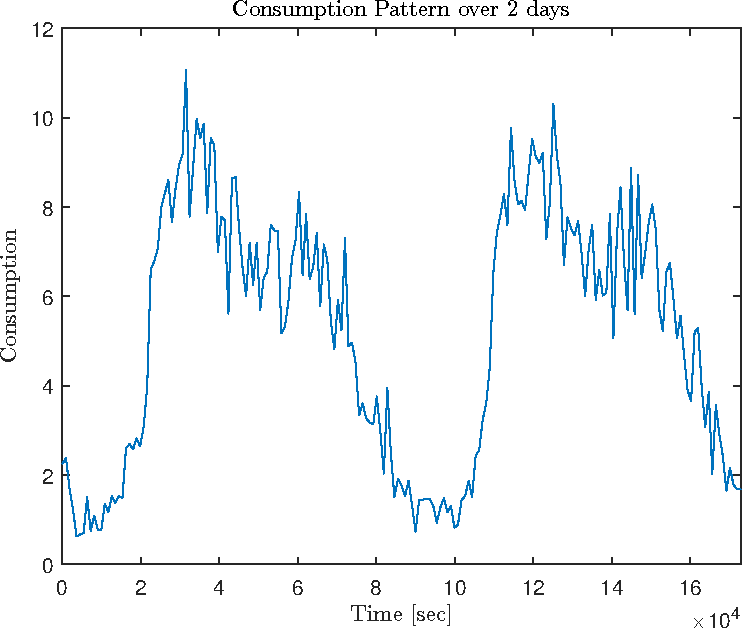
\includegraphics[width=0.8\textwidth]{Pictures/ConsumptionPattern.pdf}
	
	\caption{Consumption pattern over two days}
	\label{fig:Consumptionpattern}
\end{figure}

\begin{figure}[h!]
	\centering
	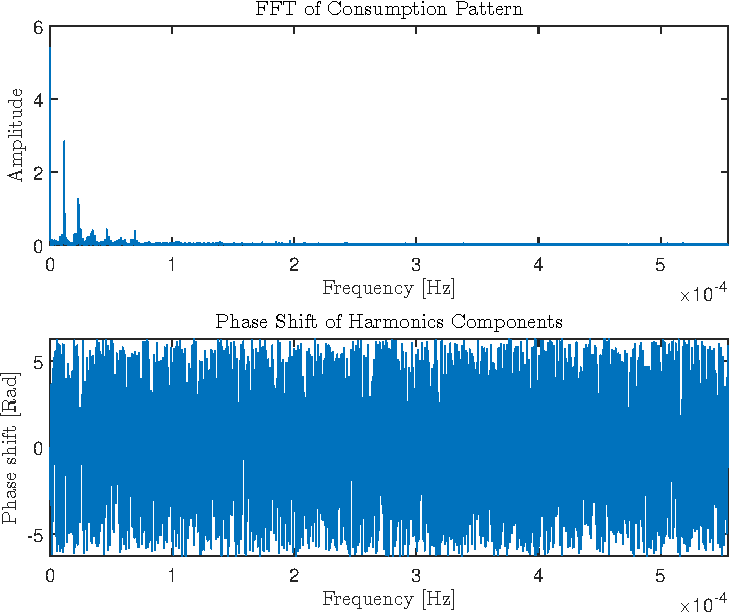
\includegraphics[width=0.8\textwidth]{Pictures/FFT.pdf}
	
	\caption{FFT results on consumption pattern}
	\label{fig:FFT}
\end{figure}

FFT analysis yields amplitude and phase plots as seen in \cref{fig:FFT}. The amplitude plot clearly shows a bias and the most influential components. To construct the correct signal we also need to identify the phase shift of each component. These can be extracted from the phase plot by identifying which indices correspond to the largest-amplitude frequency components.

\begin{figure}[h!]
	\centering
	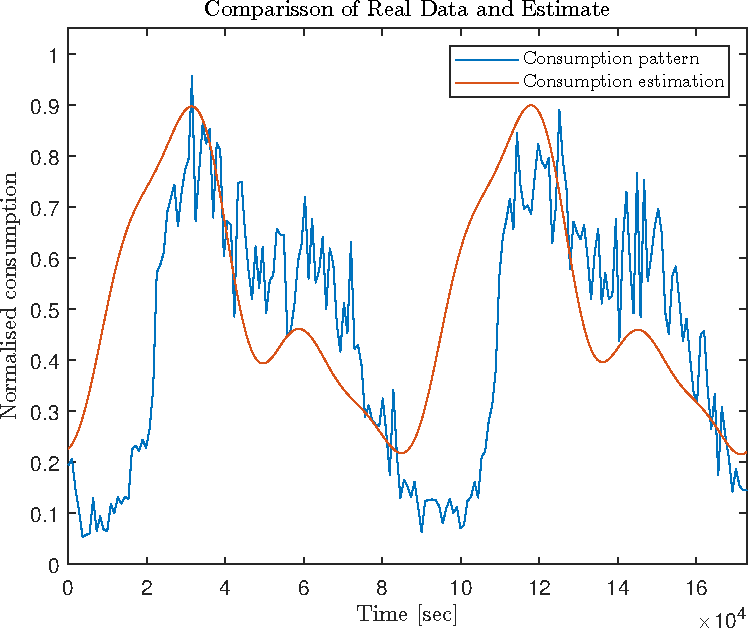
\includegraphics[width=0.8\textwidth]{Pictures/Comparisson.pdf}
	
	\caption{Comparison of raw historical data, and model}
	\label{fig:Comparison}
\end{figure}

The resulting model is compared to the raw historical data in \cref{fig:Comparison}, showing moderate coincidence. Estimate accuracy in a specific application will benefit from more thorough design of the model, possibly including additional harmonics and season-specific consumption data from the local area. Therefore, we are satisfied with the model as a general example of a consumer pattern, without requirements on validity or application. A minor correction is made based on visual inspection of the plot, resulting in a slight timeshift of the entire model to match peaks of the fundamental frequency. This is done to make up for the lack of timeshift information from the FFT.

Simulations of the Kalman filter allows us to verify its ability to track the model and simultaneously allows us to make initial guesses on covariance matrices. We have established that a model may accurately represent consumer patterns and therefore allow the estimator to place greater trust in the model than the measurements. This also improves our ability to detect a leakage, as the error between estimate and measurement becomes more prominent when the model is the primary contributor in the filter. This leads to somewhat arbitrary initial covariance guesses where the consumer model is trusted ten times more than the measurement.



\begin{figure}[h!]
	\centering
	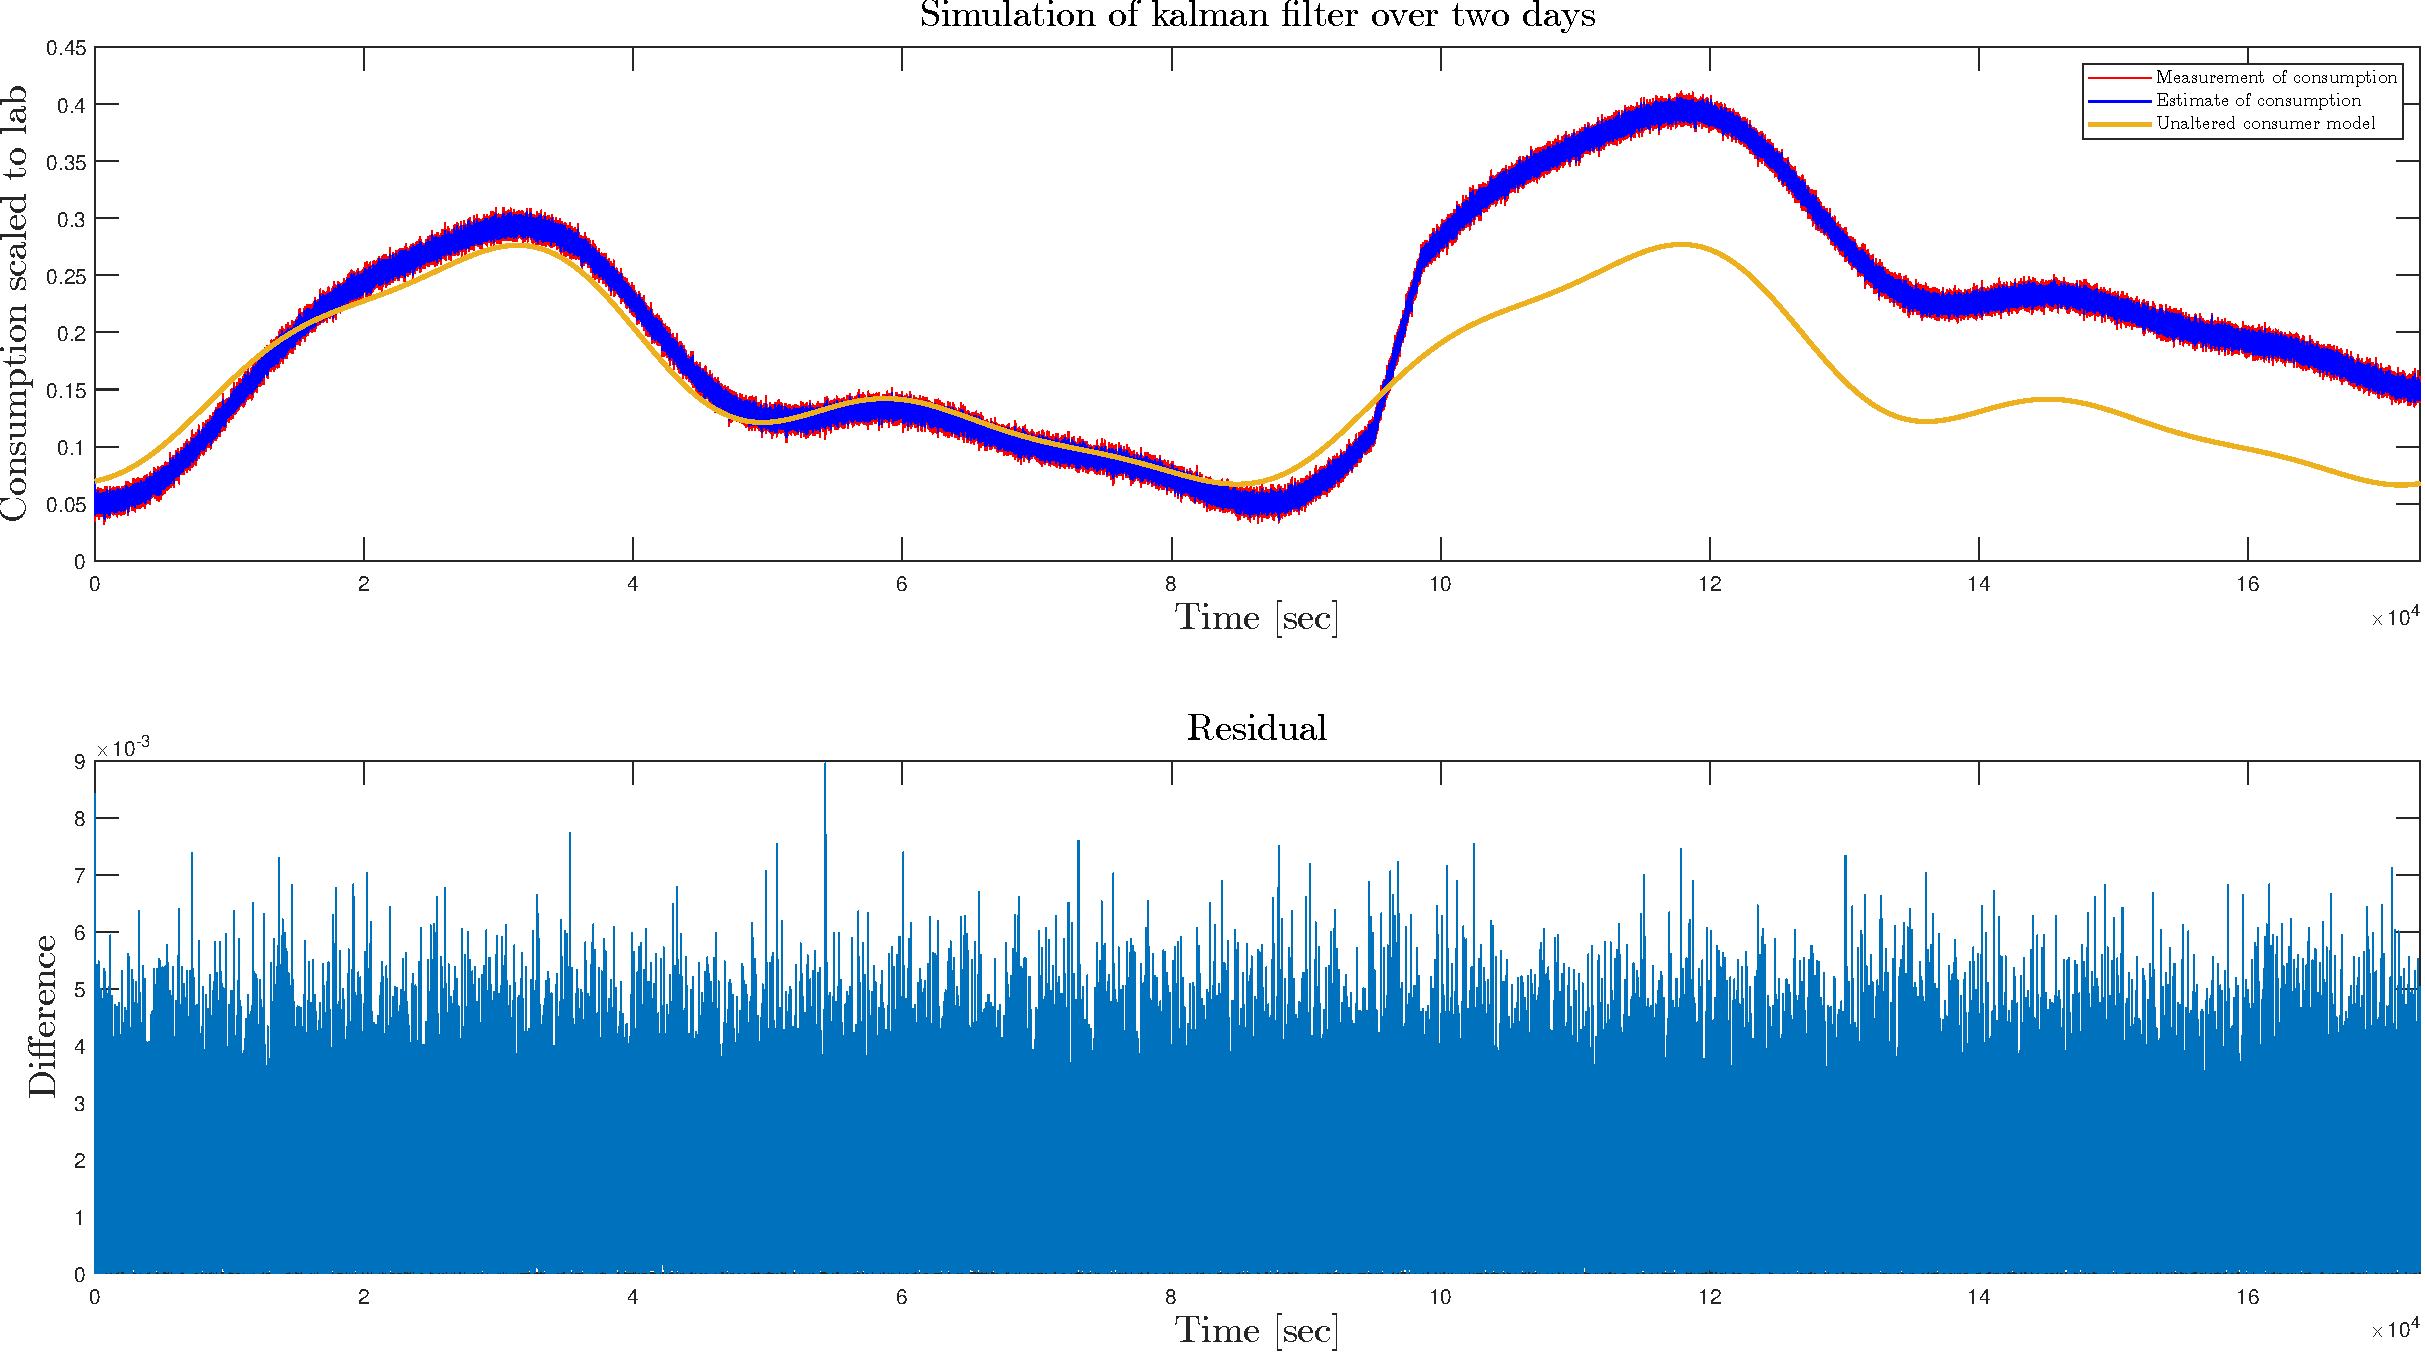
\includegraphics[width=0.8\textwidth]{Pictures/Kalman_and_Residual_Q01_R1.pdf}
	
	\caption{Simulation of the Kalman filter over two days where Q = 0.1 and R = 1.}
	\label{fig:Kalman_residual_Q01R1}
\end{figure}


A large white noise is applied to the signal; we assume this noise to be much greater than any practical occurrence, and therefore assume the filter will perform better than simulation results in any real application. The model from which measurements are drawn is also altered to simulate a discrepancy between Kalman model and real measurements. This alteration is introduced by increasing amplitude of the first two sinusoidal components by $20\%$, and reducing the third by $50\%$.

First plot in \cref{fig:Kalman_residual_Q01R1} shows the altered and unaltered model, the Kalman estimate and a leak introduced at $t = 95000$. Using covariance values $(R = 0.1, Q = 1)$, the Kalman filter tracks the altered model accurately, but it preserves a lot of noise. As such we wish to decrease our trust in measurement; this is also advantageous in terms of detecting the leak, as deviation from the expected behaviour given by the model is concealed because the filter tracks the deviation too well. This phenomenon introduces a tradeoff where we wish to accurately estimate the consumer pattern, i.e. trust measurements, such that minor changes in the pattern are tracked, and still rely enough on the model to make larger deviations stand out. The residual is shown in the second plot of \cref{fig:Kalman_residual_Q01R1}, which depicts this relationship between model accuracy and ability to detect a leak. We want to find a $Q$ value such that the plot shows a clear residual increase during the leak while retaining good tracking during periods without a leak. 

\begin{figure}[h!]
	\centering
	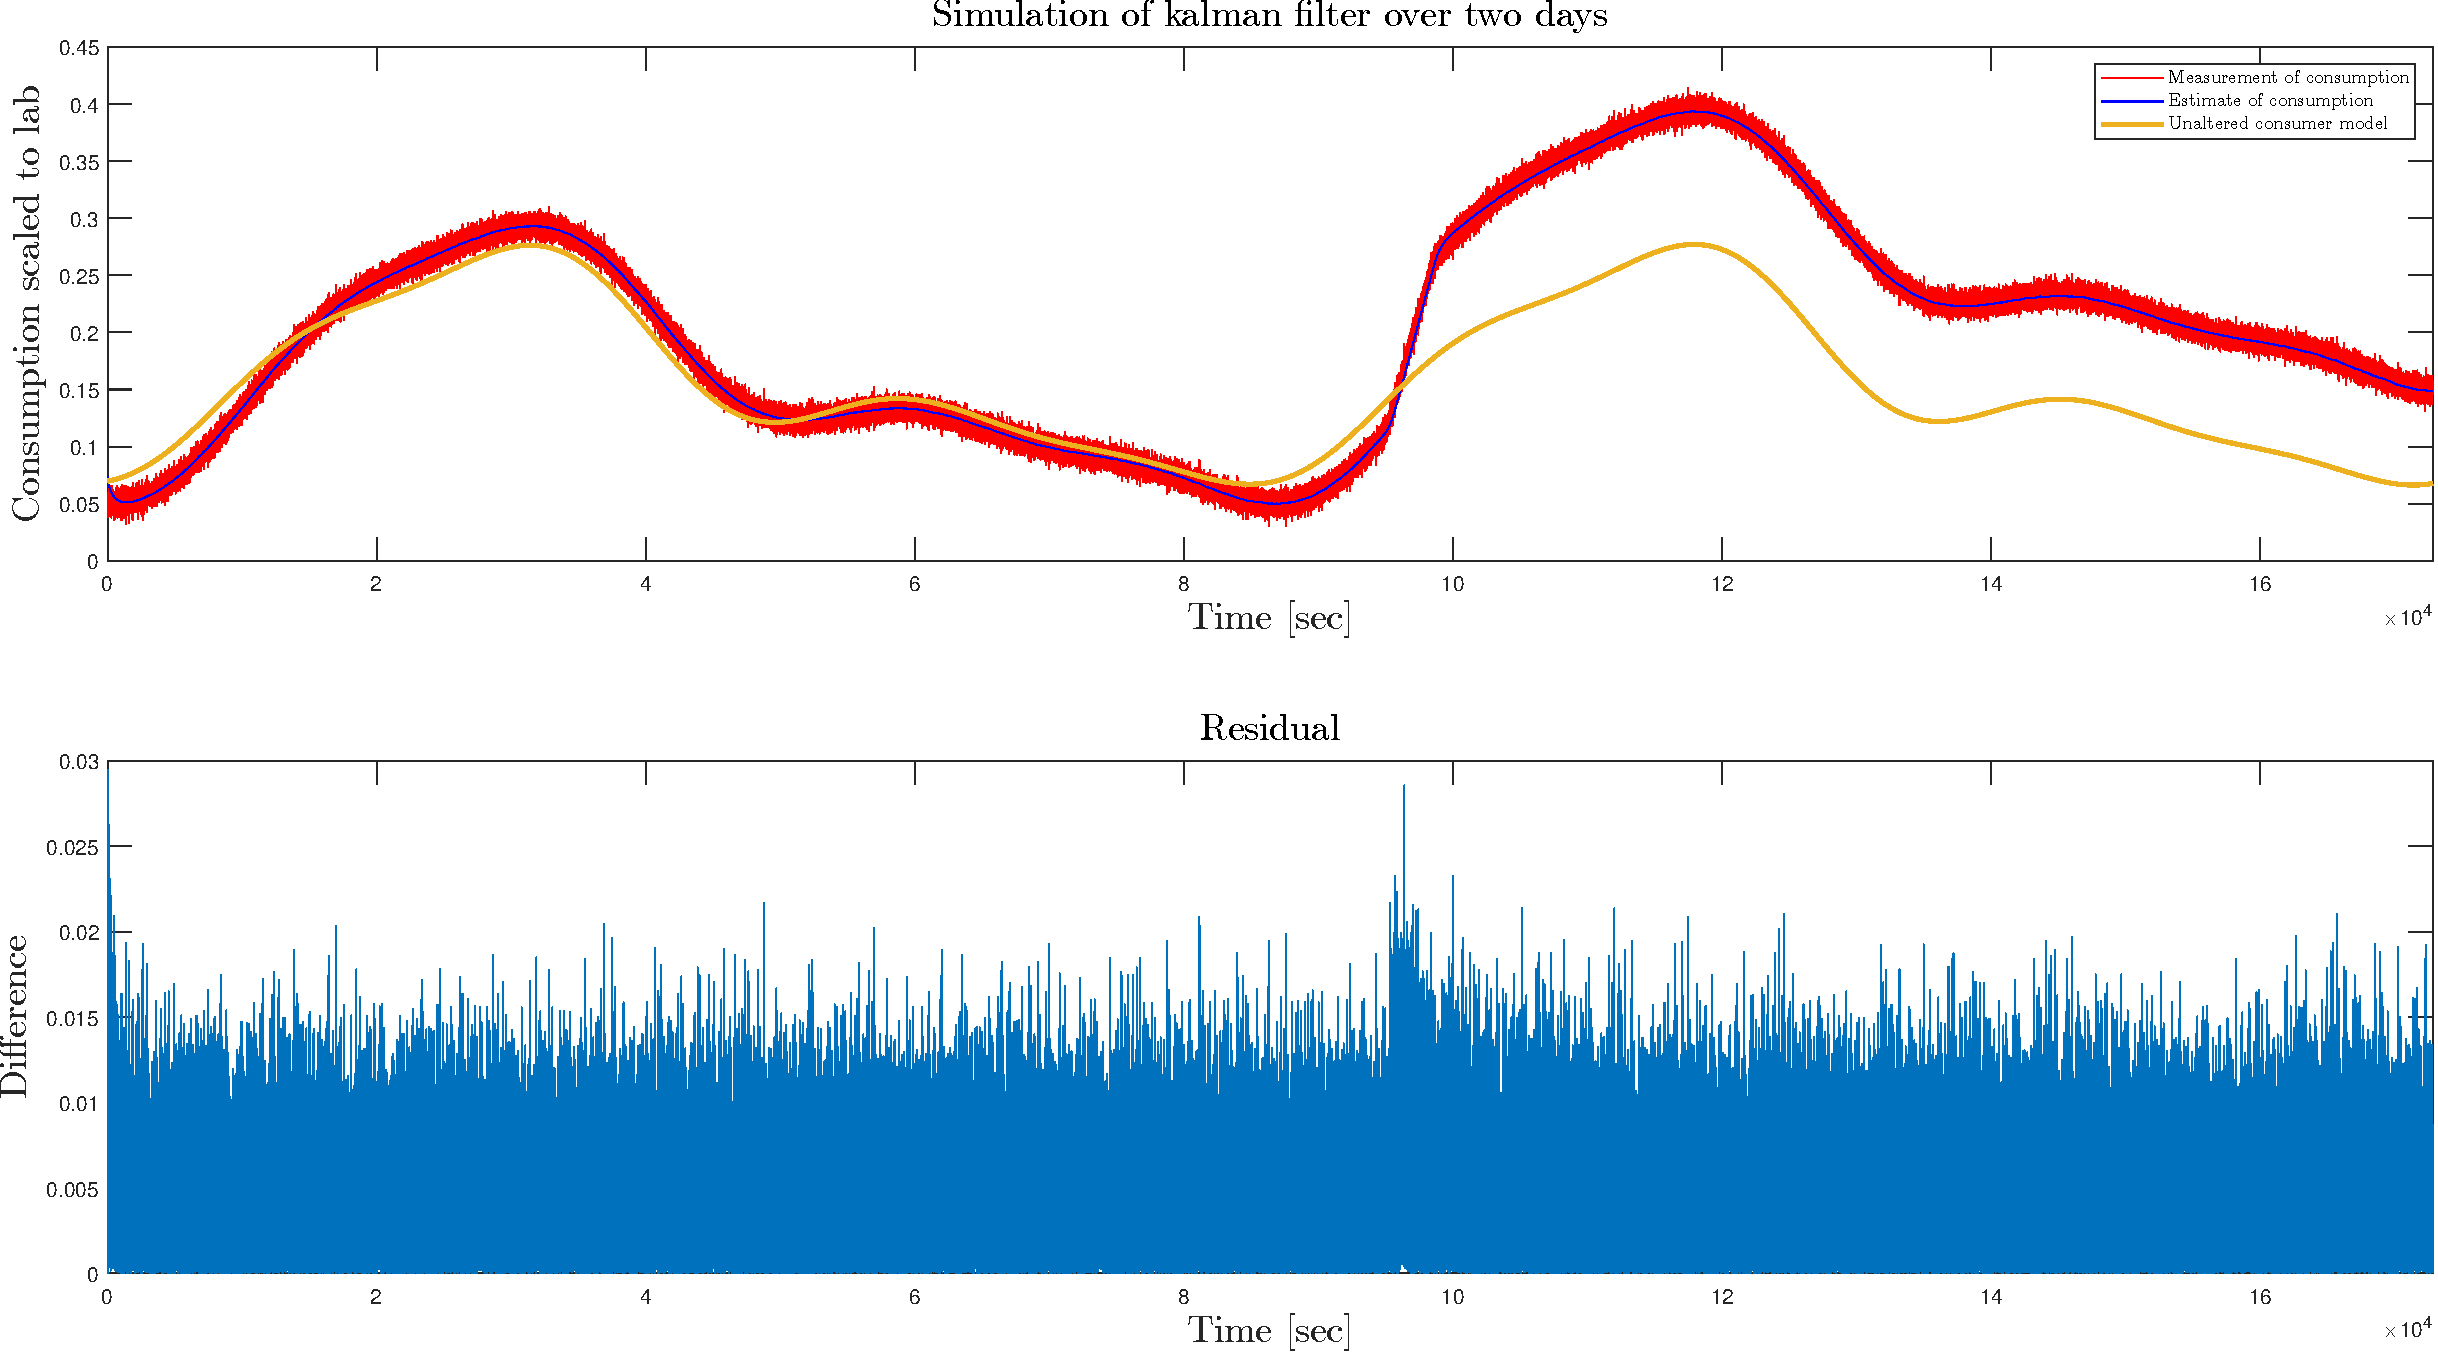
\includegraphics[width=0.8\textwidth]{Pictures/Kalman_and_Residual_Q01_R100000.pdf}
	
	\caption{Simulation of the Kalman filter over two days where Q = 0.1 and R = 100000.}
	\label{fig:Kalman_residual_Q01R100000}
\end{figure}

Increasing to $Q = 100000$ yields \cref{fig:Kalman_residual_Q01R100000}, where the slow dynamics of the consumer pattern is still tracked, and the residual plot shows a noticeable spike when the leak is introduced. The leak gradually develops over one hour, with a maximum magnitude equivalent to $33\%$ of max flow. Quite a large leak is chosen such that the residual tendency can be seen visually; a moving average algorithm is shown to easily find smaller leaks in the next section. 

\begin{figure}[h!]
	\centering
	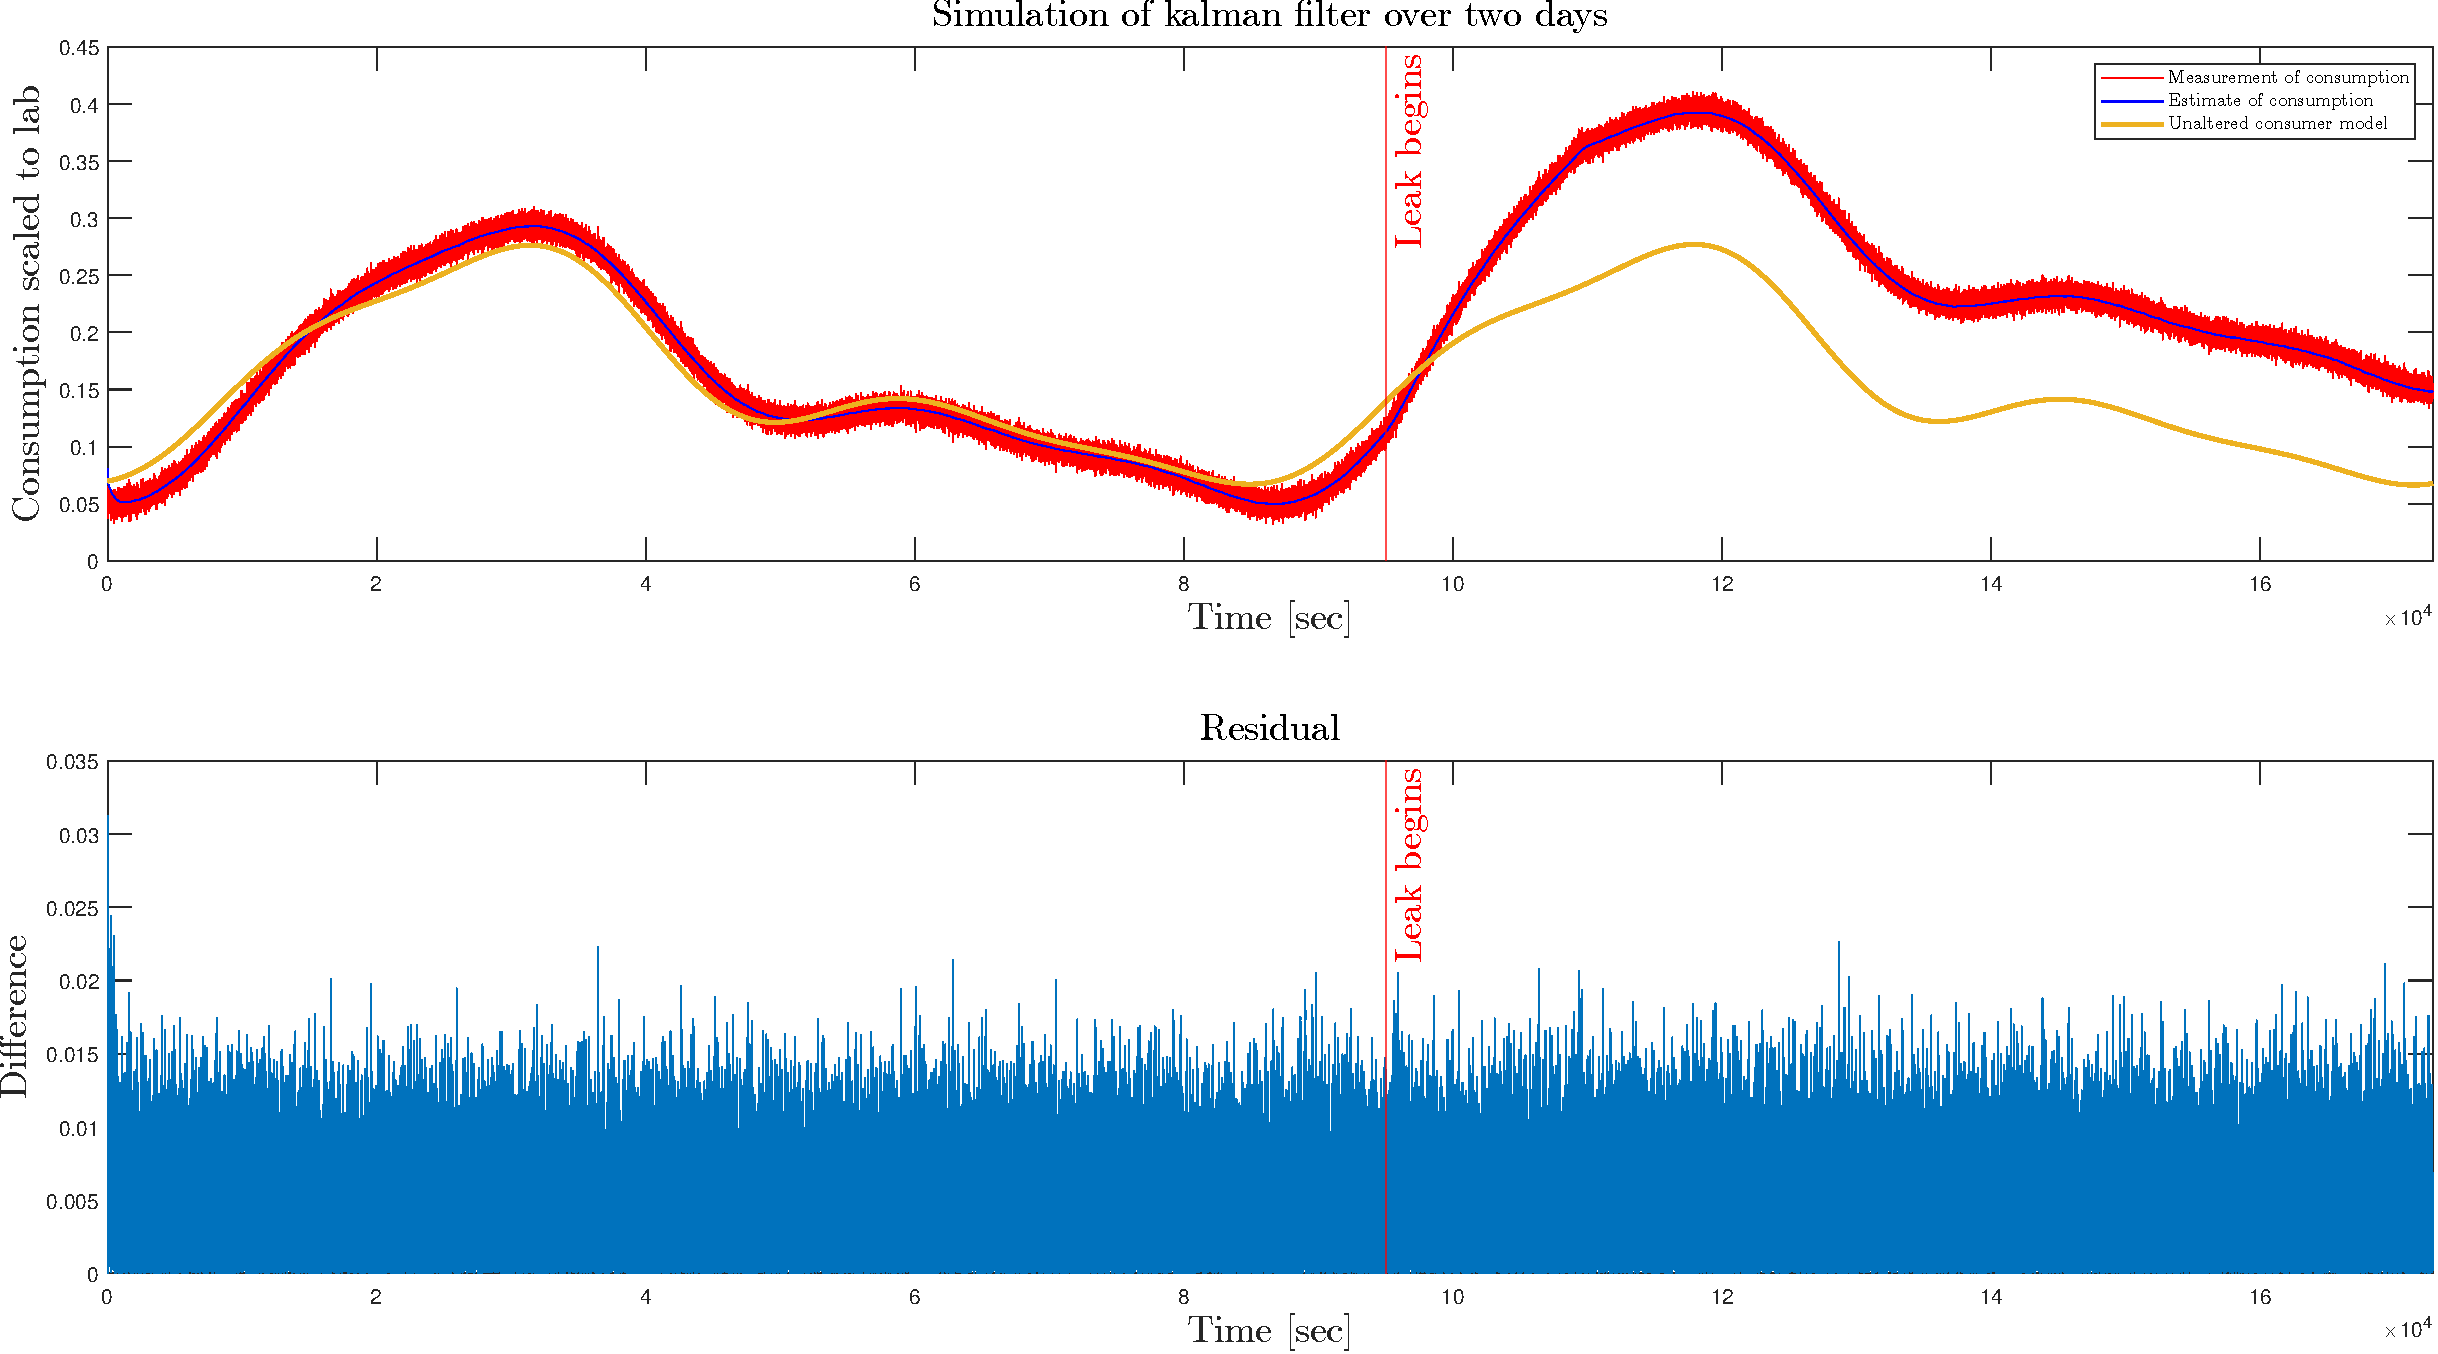
\includegraphics[width=0.8\textwidth]{Pictures/Kalman_and_Residual_Q01_R100000_4hr.pdf}
	
	\caption{Leak development slowed down to four hours.}
	\label{fig:Kalman_and_Residual_Q01_R100000_4hr}
\end{figure}

\begin{figure}[h!]
	\centering
	\includegraphics[width=0.8\textwidth]{Pictures/MA_residual_Q01_R100000_AVRG4hr.pdf}
	
	\caption{Moving average algorithm applied to residual}
	\label{fig:Movingaverage}
\end{figure}

A value of $Q = 100000$ is used in the laboratory after based on simulation results. Algorithmic leakage detection is not implemented, but we present a simple algorithm in simulation. Before proceeding, the leak is slowed down to develop over four hours instead of one, which means it will appear much more similar to the consumer model. The results are shown in \cref{fig:Kalman_and_Residual_Q01_R100000_4hr}, which also clearly shows that the leak is indistinguishable without computer processing. \cref{fig:Movingaverage} shows a moving average algorithm which computes the average residual over two hours. The figure clearly shows the average residual increasing after the leak, and a threshold could be set to automatically detect a leak. The beginning of the plot should be disregarded as it is distorted due to lacking prior information for the moving average algorithm, and the Kalman estimate needs time to settle.

In conclusion, we are confident that a leak can be detected using this method. The nature of the leak, in terms of magnitude and development is, however, important. A fast leak should be very easy to detect given the high contrast to the slow dynamics of the consumer pattern. As such, we consider a slowly developing leak. The effectiveness of this method depends on a series of variables: the correctness of the model, leak properties, and magnitude of measurement noise. We have made assumptions on these variables considering a general proof of concept, which suggests this method will work adequately for many applications, but acknowledge the importance of knowing the relevant variables.